\documentclass{izpit}

\begin{document}

%==========================================================================
%               Sem vpisi stevila tock in bo latex naracunal procente
%==========================================================================
\FRACTIONSIMPLIFY{25}{1}{\tockeprve}{\nepomembno}% zal se v paketu ne da enostavneje shraniti
\FRACTIONSIMPLIFY{20}{1}{\tockedruge}{\nepomembno}
\FRACTIONSIMPLIFY{16}{1}{\tocketretje}{\nepomembno}
%\FRACTIONSIMPLIFY{10}{1}{\tockecetrte}{\divd}%ce dodajamo dodatno nalogo
\MAX{0.1}{0}{\tempepsilon}%shranimo epsilon... ne gre trik z ulomkom zato max
\ADD{\tockeprve}{\tockedruge}{\skupnotock}
\ADD{\skupnotock}{\tocketretje}{\skupnotock}
%\ADD{\skupnotock}{\tockecetrte}{\skupnotock}%ce dodajamo dodatno nalogo
\DIVIDE{\skupnotock}{10}{\sol}
\MULTIPLY{\sol}{9}{\odlicno}
\MULTIPLY{\sol}{7.6}{\pravdobro}
\MULTIPLY{\sol}{6.3}{\dobro}
\MULTIPLY{\sol}{5}{\zadostno}
\ADD{\dobro}{\tempepsilon}{\dobroplus}%dodajanje epsilonov v spodnje meje
\ADD{\pravdobro}{\tempepsilon}{\pravdobroplus}
\ADD{\odlicno}{\tempepsilon}{\odlicnoplus}
\ROUND[1]{\dobroplus}{\dobroplus}%zaokrozevanje
\ROUND[1]{\pravdobroplus}{\pravdobroplus}
\ROUND[1]{\odlicnoplus}{\odlicnoplus}
\ROUND[1]{\zadostno}{\zadostno}
\ROUND[1]{\dobro}{\dobro}
\ROUND[1]{\pravdobro}{\pravdobro}
\ROUND[1]{\odlicno}{\odlicno}
%==========================================================================
%               Sem vpisi podatke o izpitu (ucilnica = RAZRED ali JEDILNICA)
%==========================================================================
\izpit[ucilnica = RAZRED, naloge = 3, brez vpisne]%ucilnica RAZRED,JEDILNICA, lahko se sedezni red
  {Diskretna algebraična analiza: 2. izpit}{11. 12. 2013}{
  Cas pisanja je 45 minut. Mozno je doseci $\skupnotock$ tock. Veliko uspeha!}
  
  
  \begin{flushright}
  \begin{tabular}{ll}
    \multicolumn{2}{c}{\textbf{Kriterij ocenjevanja
}} \\[0.5ex]
    Ocena & Tocke \\ \hline
    zadostno & $\zadostno - \dobro$ \\
    dobro & $\dobroplus - \pravdobro$ \\
    prav dobro & $\pravdobroplus - \odlicno$ \\
    odlicno & $\odlicnoplus$--
  \end{tabular}
  \end{flushright}
%==========================================================================
%               Sem vpisi naloge
%   za dodatek koordinatnega sistema daj pod navodila naloge \[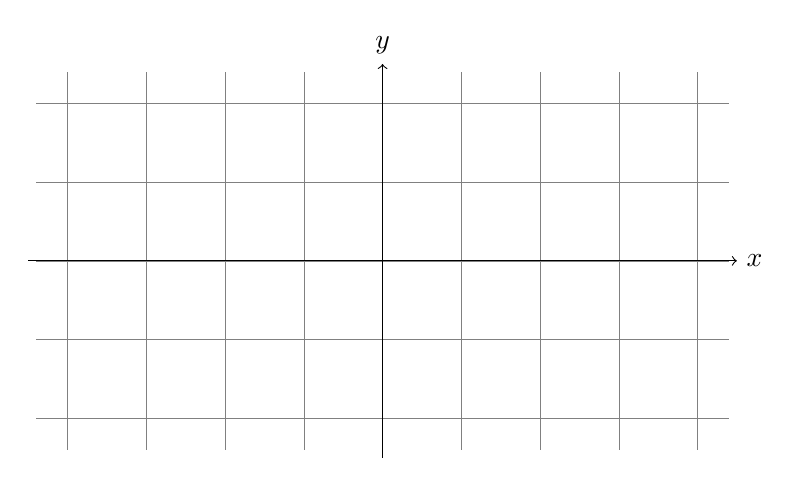
\begin{tikzpicture}
        \draw[help lines,step=1cm] (-4.4,-2.4) grid (4.4,2.4);
        \draw[->] (-4.5,0) -- (4.5,0) node[right] {$x$};
        \draw[->] (0,-2.5) -- (0,2.5) node[above] {$y$};
\end{tikzpicture}\]
%   oz. za kompleksno ravnino \[\begin{tikzpicture}
        \draw[help lines,step=1cm] (-4.4,-2.4) grid (4.4,2.4);
        \draw[->] (-4.5,0) -- (4.5,0) node[right] {$Re$};
        \draw[->] (0,-2.5) -- (0,2.5) node[above] {$Im$};
\end{tikzpicture}\]
%==========================================================================
  
\naloga[\tocke{$\tockeprve$}]

\[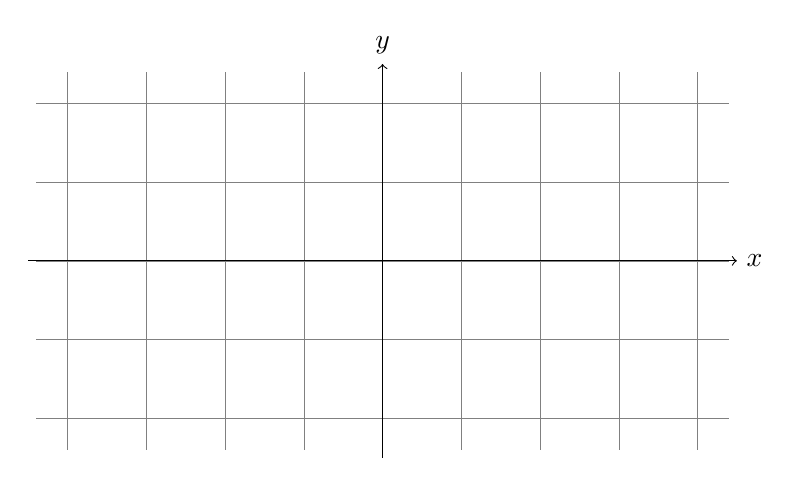
\begin{tikzpicture}
        \draw[help lines,step=1cm] (-4.4,-2.4) grid (4.4,2.4);
        \draw[->] (-4.5,0) -- (4.5,0) node[right] {$x$};
        \draw[->] (0,-2.5) -- (0,2.5) node[above] {$y$};
\end{tikzpicture}\]\\
\[\begin{tikzpicture}
        \draw[help lines,step=1cm] (-4.4,-2.4) grid (4.4,2.4);
        \draw[->] (-4.5,0) -- (4.5,0) node[right] {$Re$};
        \draw[->] (0,-2.5) -- (0,2.5) node[above] {$Im$};
\end{tikzpicture}\]

\end{document}